\documentclass[12pt, titlepage]{article}

\usepackage{fullpage}
\usepackage[round]{natbib}
\usepackage{multirow}
\usepackage{booktabs}
\usepackage{tabularx}
\usepackage{graphicx}
\usepackage{float}
\usepackage{hyperref}
\hypersetup{
    colorlinks,
    citecolor=blue,
    filecolor=black,
    linkcolor=red,
    urlcolor=blue
}

 %% Comments

\usepackage{color}

\newif\ifcomments\commentstrue %displays comments
%\newif\ifcomments\commentsfalse %so that comments do not display

\ifcomments
\newcommand{\authornote}[3]{\textcolor{#1}{[#3 ---#2]}}
\newcommand{\todo}[1]{\textcolor{red}{[TODO: #1]}}
\else
\newcommand{\authornote}[3]{}
\newcommand{\todo}[1]{}
\fi

\newcommand{\wss}[1]{\authornote{blue}{SS}{#1}} 
\newcommand{\plt}[1]{\authornote{magenta}{TPLT}{#1}} %For explanation of the template
\newcommand{\an}[1]{\authornote{cyan}{Author}{#1}}

 %% Common Parts

\newcommand{\progname}{Course Buddy} % PUT YOUR PROGRAM NAME HERE
\newcommand{\authname}{Team \#5, Overwatch League
\\ Jingyao, Qin
\\ Qianni, Wang
\\ Qiang, Gao
\\ Chenwei, Song
\\ Shuting, Shi
\\ } % AUTHOR NAMES                  

\usepackage{hyperref}
    \hypersetup{colorlinks=true, linkcolor=blue, citecolor=blue, filecolor=blue,
                urlcolor=blue, unicode=false}
    \urlstyle{same}
                                

\newcounter{acnum}
\newcommand{\actheacnum}{AC\theacnum}
\newcommand{\acref}[1]{AC\ref{#1}}

\newcounter{ucnum}
\newcommand{\uctheucnum}{UC\theucnum}
\newcommand{\uref}[1]{UC\ref{#1}}

\newcounter{mnum}
\newcommand{\mthemnum}{M\themnum}
\newcommand{\mref}[1]{M\ref{#1}}

\begin{document}

\title{Module Guide for \progname{MacONE}} 
\author{\authname}
\date{\today}

\maketitle

\pagenumbering{roman}

\section{Revision History}

\begin{tabularx}{\textwidth}{p{3cm}p{2cm}X}
\toprule {\bf Date} & {\bf Version} & {\bf Notes}\\
\midrule
2024-01-17 & 1.0 & First version of module guide\\
2024-04-03 & 2.0 & Update after final demo\\
\bottomrule
\end{tabularx}

\newpage

\section{Reference Material}

This section records information for easy reference.

\subsection{Abbreviations and Acronyms}

\renewcommand{\arraystretch}{1.2}
\begin{tabular}{l l} 
  \toprule		
  \textbf{symbol} & \textbf{description}\\
  \midrule 
  AC & Anticipated Change\\
  DAG & Directed Acyclic Graph \\
  M & Module \\
  MG & Module Guide \\
  OS & Operating System \\
  SRS & Software Requirements Specification\\
  UC & Unlikely Change \\
  \wss{etc.} & \wss{...}\\
  \bottomrule
\end{tabular}\\

\newpage

\tableofcontents

\listoftables

\listoffigures

\newpage

\pagenumbering{arabic}

\section{Introduction}

Decomposing a system into modules is a commonly accepted approach to developing
software.  A module is a work assignment for a programmer or programming
team ~\cite{Parnas1972a}.  We advocate a decomposition
based on the principle of information hiding ~\citep{Parnas1972a}.  This
principle supports design for change, because the ``secrets'' that each module
hides represent likely future changes.  Design for change is valuable in SC,
where modifications are frequent, especially during initial development as the
solution space is explored.  

Our design follows the rules layed out by ~\citet{ParnasEtAl1984}, as follows:
\begin{itemize}
\item System details that are likely to change independently should be the
  secrets of separate modules.
\item Each data structure is implemented in only one module.
\item Any other program that requires information stored in a module's data
  structures must obtain it by calling access programs belonging to that module.
\end{itemize}

After completing the first stage of the design, the Software Requirements
Specification (SRS), the Module Guide (MG) is developed ~\citep{ParnasEtAl1984}. The MG
specifies the modular structure of the system and is intended to allow both
designers and maintainers to easily identify the parts of the software.  The
potential readers of this document are as follows:

\begin{itemize}
\item New project members: This document can be a guide for a new project member
  to easily understand the overall structure and quickly find the
  relevant modules they are searching for.
\item Maintainers: The hierarchical structure of the module guide improves the
  maintainers' understanding when they need to make changes to the system. It is
  important for a maintainer to update the relevant sections of the document
  after changes have been made.
\item Designers: Once the module guide has been written, it can be used to
  check for consistency, feasibility, and flexibility. Designers can verify the
  system in various ways, such as consistency among modules, feasibility of the
  decomposition, and flexibility of the design.
\end{itemize}

The rest of the document is organized as follows. Section
\ref{SecChange} lists the anticipated and unlikely changes of the software
requirements. Section \ref{SecMH} summarizes the module decomposition that
was constructed according to the likely changes. Section \ref{SecConnection}
specifies the connections between the software requirements and the
modules. Section \ref{SecMD} gives a detailed description of the
modules. Section \ref{SecTM} includes two traceability matrices. One checks
the completeness of the design against the requirements provided in the SRS. The
other shows the relation between anticipated changes and the modules. Section
\ref{SecUse} describes the use relation between modules.

\section{Anticipated and Unlikely Changes} \label{SecChange}

This section lists possible changes to the system. According to the likeliness
of the change, the possible changes are classified into two
categories. Anticipated changes are listed in Section \ref{SecAchange}, and
unlikely changes are listed in Section \ref{SecUchange}.

\subsection{Anticipated Changes} \label{SecAchange}

Anticipated changes are the source of the information that is to be hidden
inside the modules. Ideally, changing one of the anticipated changes will only
require changing the one module that hides the associated decision. The approach
adapted here is called design for
change.

\begin{description}
\item[\refstepcounter{acnum} \actheacnum \label{acUI}:]
The user interface design could be changed, especially the layout, colour, and fonts.
\item[\refstepcounter{acnum} \actheacnum \label{acALGM}:]
The algorithms might be changed, such as the algorithm for PDF extraction and task priority prediction.
\item[\refstepcounter{acnum} \actheacnum \label{acDBSCH}:]
The database storage system could be modified, such as the database schema, tables, constraints or other elements.
\item[\refstepcounter{acnum} \actheacnum \label{acAPI}:]
The API usage in the back-end system could be upgraded or changed.
\item[\refstepcounter{acnum} \actheacnum \label{acSCALE}:]
The web load or data scale could be changed in the development of the application.

\end{description}

\subsection{Unlikely Changes} \label{SecUchange}

The module design should be as general as possible. However, a general system is
more complex. Sometimes this complexity is not necessary. Fixing some design
decisions at the system architecture stage can simplify the software design. If
these decisions should later need to be changed, then many parts of the design
will potentially need to be modified. Hence, it is not intended that these
decisions will be changed.

\begin{description}
\item[\refstepcounter{ucnum} \uctheucnum \label{ucIO}:] The programming languages and technical stack won't be changed.
\item[\refstepcounter{ucnum} \uctheucnum \label{ucIO}:] The major functionality and purpose of this application won't be changed from educational use to other business use.  
\item[\refstepcounter{ucnum} \uctheucnum \label{ucIO}:]
The deployment of the database on AWS cloud service won't be changed because of high cost.
\item[\refstepcounter{ucnum} \uctheucnum \label{ucIO}:] The application's overall architecture won't be changed dramatically.
\item[\refstepcounter{ucnum} \uctheucnum \label{ucIO}:]
The interface device would always be the computer keyboard and monitor.
\end{description}

\section{Module Hierarchy} \label{SecMH}

This section provides an overview of the module design. Modules are summarized
in a hierarchy decomposed by secrets in Table \ref{TblMH}. The modules listed
below, which are leaves in the hierarchy tree, are the modules that will
actually be implemented.

\begin{description}
\item [\refstepcounter{mnum} \mthemnum \label{mIM}:] Interface Module
\item [\refstepcounter{mnum} \mthemnum \label{mBEWS}:] Back End Web Service Module
\item [\refstepcounter{mnum} \mthemnum \label{mUserAM}:] User Authentication Module
\item [\refstepcounter{mnum} \mthemnum \label{mAGM}:] App Grid Module
\item [\refstepcounter{mnum} \mthemnum \label{mTaskAM}:] Task Module
\item [\refstepcounter{mnum} \mthemnum \label{mCM}:] Course Module
\item [\refstepcounter{mnum} \mthemnum \label{mUM}:] User Module
\item [\refstepcounter{mnum} \mthemnum \label{mPM}:] Pomodoro Module
\item [\refstepcounter{mnum} \mthemnum \label{mFM}:] Forum Module
\item [\refstepcounter{mnum} \mthemnum \label{mFBM}:] Feedback Module
\item [\refstepcounter{mnum} \mthemnum \label{mPEM}:] PDF Extraction Module
\item [\refstepcounter{mnum} \mthemnum \label{mCCM}:] cGPA Calculation Module
\item [\refstepcounter{mnum} \mthemnum \label{mDTM}:] Database Module
\end{description}


\begin{table}[h!]
\centering
\begin{tabular}{p{0.3\textwidth} p{0.6\textwidth}}
\toprule
\textbf{Level 1} & \textbf{Level 2}\\
\midrule

{Hardware-Hiding Module} & Interface Module\\
\midrule

\multirow{7}{0.3\textwidth}{Behaviour-Hiding Module}
& Back End Web Service Module\\
& User Authentication Module\\ 
& App Grid Module Module\\ 
& Task Module\\
& Course Module\\
& User Module\\
& Pomodoro Module\\
& Forum Module\\
& Feedback Module\\
\midrule

\multirow{3}{0.3\textwidth}{Software Decision Module}
& PDF Extraction Module \\
& cGPA Calculation Module \\
& Database Module\\

\bottomrule

\end{tabular}
\caption{Module Hierarchy}
\label{TblMH}
\end{table}

\newpage
\section{Connection Between Requirements and Design} \label{SecConnection}

The design of the system is intended to satisfy the requirements developed in
the SRS. In this stage, the system is decomposed into modules. The connection
between requirements and modules is listed in Table~\ref{TblRT}.

\section{Module Decomposition} \label{SecMD}

Modules are decomposed according to the principle of ``information hiding''
proposed by \citet{ParnasEtAl1984}. The \emph{Secrets} field in a module
decomposition is a brief statement of the design decision hidden by the
module. The \emph{Services} field specifies \emph{what} the module will do
without documenting \emph{how} to do it. For each module, a suggestion for the
implementing software is given under the \emph{Implemented By} title

Only the leaf modules in the hierarchy have to be implemented. If a dash
(\emph{--}) is shown, this means that the module is not a leaf and will not have
to be implemented.

\subsection{Hardware Hiding Modules }

\subsubsection{Interface Module (\mref{mIM})}
\begin{description}
\item[Secrets:]Hide the detailed structure and logic of front-end technical implementation, which involves the graphic design and user interface.
\item[Services:]Serves as the medium for users to interact with the application to implement diverse functionalities effectively. The client side of the application sends user data to the backend, and then in turn processes the received information and displays it in the interface in a user-friendly and easily understandable form. 
\item[Implemented By:] Developed using web technologies like HTML, CSS

\end{description}

\subsection{Behaviour-Hiding Module}

\begin{description}
\item[Secrets:]The contents of the required behaviours.
\item[Services:]Includes programs that provide externally visible behaviour of
  the system as specified in the software requirements specification (SRS)
  documents. This module serves as a communication layer between the
  hardware-hiding module and the software decision module. The programs in this
  module will need to change if there are changes in the SRS.
\item[Implemented By:] --
\end{description}

\subsubsection{Back End Web Service Module (\mref{mBEWS})}

\begin{description}
\item[Secrets:] Internal Logic and data processing methods
\item[Services:] Offers web services for front-end modules, handling requests, responses and exceptions
\item[Implemented By:] Server-side Languages and Principles
\end{description}


\subsubsection{User Authentication Module (\mref{mUserAM})}

\begin{description}
\item[Secrets:] The confidential authentication mechanism, involves the encryption of the password, the location of data stored, and the process of verification of data.
\item[Services:]  Provides verification service for checking user identities during the login procedure. This module ensures only the authenticated user can access certain features of this application.
\item[Implemented By:] Integrates with User Module and Database module, utilizes data mapping and hashing technique for verification. 
\end{description}

\subsubsection{App Grid Module (\mref{mAGM})}

\begin{description}
\item[Secrets:] The categorization and manipulation of apps.
\item[Services:] Provides functionalities for users to change the position of icons in the app grid.
\item[Implemented By:] Integrates with the database module for consistent data storage of app grid information.
\end{description}

\subsubsection{Task Module (\mref{mTaskAM})}

\begin{description}
\item[Secrets:] The categorization and manipulation of tasks.
\item[Services:] Provides functionalities for users to manipulate tasks, including creating, reading, updating and deleting tasks. Also, the service involves additional features: setting deadlines,  tasks, set difficulty levels. 
\item[Implemented By:] Integrates with the database module for consistent data storage of task information. Also, utilize request transmission technique API for sending data to the Task prioritization module, and receive requests from the back-end server-side to execute instructions.
\end{description}


\subsubsection{Course Module (\mref{mCM})}

\begin{description}
\item[Secrets:]Course Data structure and management algorithms
\item[Services:]Manages course information, including the creation, modification, and deletion.
\item[Implemented By: Integrates with the database for storing the course data] 
\end{description}

\subsubsection{User Module (\mref{mUM})}

\begin{description}
\item[Secrets:] User info data handling method.
\item[Services:] Manages User information, including the creation, modification, and deletion.
\item[Implemented By:] Integrates with the database module and authentication module. 
\end{description}


\subsubsection{Pomodoro Module (\mref{mPM})}

\begin{description}
\item[Secrets:] Specific study time interval and design technique
\item[Services:] Provides a Pomodoro timer for users productively conduct study tasks. 
\item[Implemented By:] Integrate with the user interface and provide a real-time interactive feature by scripting language and UI design.
\end{description}

\subsubsection{Forum Module (\mref{mFM})}

\begin{description}
\item[Secrets:] Forum info data handling method.
\item[Services:] Manages forum information, including the creation, modification, and deletion.
\item[Implemented By:] Integrate with the user interface and provide a real-time interactive feature by scripting language and UI design.
\end{description}

\subsubsection{Feedback Module (\mref{mFBM})}

\begin{description}
\item[Secrets:] Feedback info data handling method.
\item[Services:] Manages feedback information, including the creation and modification.
\item[Implemented By:] Integrates with the database module and UI design.
\end{description}

\subsection{Software Decision Module}

\begin{description}
\item[Secrets:] The design decision based on mathematical theorems, physical
  facts, or programming considerations. The secrets of this module are
  \emph{not} described in the SRS.
\item[Services:] Includes data structure and algorithms used in the system that
  do not provide direct interaction with the user. 
  % Changes in these modules are more likely to be motivated by a desire to
  % improve performance than by externally imposed changes.
\item[Implemented By:] --
\end{description}


\subsubsection{PDF Extraction Module (\mref{mPEM})}

\begin{description}
\item[Secrets:] Techniques and specific algorithms or logics for extracting data from PDF files, and the standardized format of data while to be stored in the database. 
\item[Services:] Extracts and processes information from the user-uploaded PDF documents.
\item[Implemented By:] Utilizes specific libraries for pdf processing
\end{description}

\subsubsection{cGPA Calculation Module (\mref{mCCM})}

\begin{description}
\item[Secrets:] Techniques and specific algorithms or logics for calculating cGpa from PDF files. 
\item[Services:] Extracts and processes information from the user-uploaded PDF documents.
\item[Implemented By:] Utilizes specific libraries for pdf processing
\end{description}

\subsubsection{Database Module (\mref{mDTM})}

\begin{description}
\item[Secrets:] Database schema and query optimization techniques
\item[Services:] Provides CRUD (create, read, update, and delete) manipulation of all the data used in the application efficiently. 
\item[Implemented By:] Deployed on the AWS cloud service platform and utilized a relational database system.  
\end{description}

\section{Traceability Matrix} \label{SecTM}

This section shows two traceability matrices: between the modules and the
requirements and between the modules and the anticipated changes.

The traceability between NFR and Modules is not provided, as the majority of NFRs are only associated with the Interface Module(\mref{mCM}).  The current design and development practices already mitigate the most critical NFRs (such as using a responsive framework for UI development), detailed traceability for each NFR may not provide additional value at this stage.

% the table should use mref, the requirements should be named, use something
% like fref
\begin{table}[H]
\centering
\begin{tabular}{p{0.2\textwidth} p{0.6\textwidth}}
\toprule
\textbf{Req.} & \textbf{Modules}\\
\midrule
FR1 & \mref{mCM}, \mref{mBEWS}, \mref{mPEM} \mref{mDTM}\\
FR2 & \mref{mCM}, \mref{mTaskAM}, \mref{mPM}, \mref{mBEWS}, \mref{mDTM}\\
FR3 & \mref{mUM}, \mref{mCM}, \mref{mBEWS}, \mref{mDTM}, \mref{mTaskAM}\\
FR4 & \mref{mUM}, \mref{mCM}, \mref{mBEWS}, \mref{mDTM}, \mref{mTaskAM}\\
FR5 & \mref{mUM}, \mref{mBEWS}, \mref{mDTM}, \mref{mPM}\\
FR6 & \mref{mUM}, \mref{mBEWS}, \mref{mDTM}, \mref{mPM}\\
FR7 & \mref{mUM}, \mref{mDTM}, \mref{mPM}\\
FR8 & \mref{mUM}, \mref{mDTM}, \mref{mPM}\\
FR9 & \mref{mUM}, \mref{mDTM}, \mref{mTaskAM}, \mref{mBEWS}\\
FR10 & \mref{mIM}, \mref{mDTM}, \mref{mTaskAM}\\
FR11 & \mref{mIM}, \mref{mDTM}, \mref{mTaskAM} \mref{mBEWS}\\
FR12 & \mref{mIM}, \mref{mDTM}, \mref{mTaskAM}\\
FR13 & \mref{mIM}, \mref{mTaskAM}\\
FR14 & \mref{mUM}, \mref{mIM}, \mref{mBEWS}, \mref{mFM}, \mref{mDTM}\\
FR15 & \mref{mFM}, \mref{mDTM}\\
FR16 & \mref{mUM}, \mref{mIM}, \mref{mBEWS}, \mref{mFM}, \mref{mDTM}\\
FR17 & \mref{mUM}, \mref{mIM}, \mref{mBEWS}, \mref{mFM}, \mref{mDTM}\\
FR18 & \mref{mIM}, \mref{mUM}, \mref{mAGM}, \mref{mDTM}\\
FR19 & \mref{mIM}, \mref{mUM}, \mref{mAGM}, \mref{mDTM} \mref{mBEWS}\\
FR20 & \mref{mIM}, \mref{mFBM}, \mref{mBEWS}, \mref{mDTM}\\
FR21 & \mref{mIM}, \mref{mFBM}, \mref{mDTM}\\
FR22 & \mref{mIM}, \mref{mFBM}, \mref{mDTM}\\
FR23 & \mref{mIM}, \mref{mUserAM}, \mref{mUM}, \mref{mBEWS}, \mref{mDTM}\\
FR24 & \mref{mIM}, \mref{mBEWS}, \mref{mCCM}\\
\bottomrule
\end{tabular}
\caption{Trace Between Requirements and Modules}
\label{TblRT}
\end{table}

\begin{table}[H]
\centering
\begin{tabular}{p{0.2\textwidth} p{0.6\textwidth}}
\toprule
\textbf{AC} & \textbf{Modules}\\
\midrule
\acref{acUI} & \mref{mIM}\\
\acref{acALGM} & \mref{mCCM}, \mref{mPEM}\\
\acref{acDBSCH} & \mref{mDTM}\\
\acref{acAPI} & \mref{mBEWS}\\
\acref{acSCALE} & \mref{mDTM} \\
\bottomrule
\end{tabular}
\caption{Trace Between Anticipated Changes and Modules}
\label{TblACT}
\end{table}

\section{Use Hierarchy Between Modules} \label{SecUse}
The use hierarchy between these modules is represented using a DAG diagram, which visualizes the interconnections between different modules inside this software application system. Each node represents a module stated in the previous module decomposition section. The edges indicate the dependencies between modules. An arrow from module A to module B implies that module A depends on module B, both the functionality support and data transmission. We can see that the Back End Web Service Module is located as a central node on this diagram, which serves as a communication hub for the breach of sub-system modules.

This diagram reflects several software architecture concepts. Modularity can be easily understood, the information-hiding principle is also an additional effect.  Each module hides its internal details from other modules, and the design idea of loose coupling and high cohesion are proven. Such layer architecture makes this application can be high maintainable and reusable because the changes in one individual module would have little effect on others. 
\begin{figure}[H]
\centering
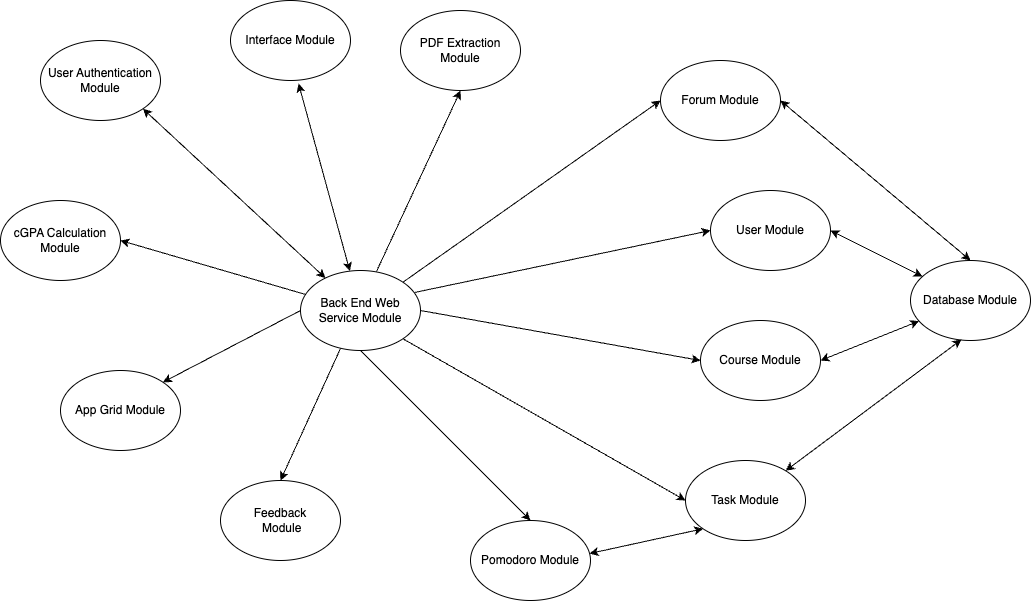
\includegraphics[width=0.7\textwidth]{UseHierachy.png}
\caption{Use hierarchy among modules}
\label{FigUH}
\end{figure}

\section{Timeline}

This section provides a detailed timeline for the implementation, testing, and verification of the system modules, split across two pages for clarity. Each task requires the collaboration of two or more team members to ensure thoroughness and accuracy. The timeline is structured to ensure functional implementation and basic testing by February 5, 2024, and complete full testing and verification by February 20, 2024.

% Part 1 of the table
\begin{table}[H]
\centering
\begin{tabular}{|p{0.15\textwidth}|p{0.35\textwidth}|p{0.25\textwidth}|p{0.15\textwidth}|}
\hline
\textbf{Module} & \textbf{Task} & \textbf{Responsible Members} & \textbf{Completion Date} \\
\hline
Interface Module & UI Design and Initial Development & Jingyao Qin, Chenwei Song & 2024-01-24 \\
\hline
 & UI Module Testing & Qianni Wang, Shuting Shi & 2024-01-28 \\
\hline
Back End Web Service & Server Setup and API Development & Chenwei Song, Qiang Gao & 2024-01-26 \\
\hline
 & Back End Module Testing & Jingyao Qin, Qianni Wang & 2024-01-30 \\
\hline
User Authentication & Authentication Mechanism Implementation & Qianni Wang, Shuting Shi & 2024-01-25 \\
\hline
 & Authentication Module Testing & Chenwei Song, Qiang Gao & 2024-01-29 \\
\hline
Task Module & Task Management Functions Implementation & Shuting Shi, Qiang Gao & 2024-01-27 \\
\hline
 & Task Module Testing & Jingyao Qin, Chenwei Song & 2024-01-31 \\
\hline
Database Module & Database Design and Integration & Qiang Gao, Jingyao Qin & 2024-01-26 \\
\hline
 & Database Module Testing & Qianni Wang, Shuting Shi & 2024-01-30 \\
\hline
Pomodoro Module & Timer Functionality Implementation & Jingyao Qin, Qianni Wang & 2024-01-23 \\
\hline
 & Pomodoro Module Testing & Chenwei Song, Qiang Gao & 2024-01-27 \\
\hline
PDF Extraction Module & PDF Processing and Extraction Logic & Chenwei Song, Shuting Shi & 2024-01-28 \\
\hline
 & PDF Extraction Module Testing & Qianni Wang, Qiang Gao & 2024-02-01 \\
\hline
Feedback Module & App order Functions Implementation & Qianni Wang & 2024-01-27 \\
\hline
 & Feedback Module Testing & Jingyao Qin, Chenwei Song & 2024-01-31 \\
\hline
cGpa calculation Module & App order Functions Implementation & Qianni Wang & 2024-01-27 \\
\hline
 & cGpa calculation Module Testing & Jingyao Qin, Chenwei Song & 2024-01-31 \\
\hline
\end{tabular}
\caption{Timeline (Part 1)}
\label{table:timeline1}
\end{table}
\newpage 

\begin{table}[H]
\centering
\begin{tabular}{|p{0.15\textwidth}|p{0.35\textwidth}|p{0.25\textwidth}|p{0.15\textwidth}|}
\hline
\textbf{Module} & \textbf{Task} & \textbf{Responsible Members} & \textbf{Completion Date} \\
\hline
App grid Module & App order Functions Implementation & Qianni Wang & 2024-01-27 \\
\hline
 & App grid Module Testing & Jingyao Qin, Chenwei Song & 2024-01-31 \\
\hline
Forum Module & App order Functions Implementation & Chenwei Song & 2024-01-27 \\
\hline
 & Forum Module Testing &Chenwei Song & 2024-01-31 \\
\hline
Basic Testing & Integration Testing for Each Module & All Members & 2024-02-05 \\
\hline
Refinement & Bug Fixing and Code Refinement & All Members & 2024-02-10 \\
\hline
Full Testing and Verification & Comprehensive System Testing & All Members & 2024-02-15 \\
\hline
Final Verification & Final Review and Verification & All Members & 2024-02-20 \\
\hline
\end{tabular}
\caption{Timeline (Part 2)}
\label{table:timeline2}
\end{table}




\section{Reflection}
The information in this section will be used to evaluate the team members on the
graduate attribute of Problem Analysis and Design.  Please answer the following questions:

\begin{enumerate}
  \item What are the limitations of your solution?  Put another way, given
  unlimited resources, what could you do to make the project better? (LO\_ProbSolutions)

  The current scope of our application is very limited because of the cost consideration. If the user amount grows significantly, our backend module may face the condition of overload, and traffic burden. Also, The central module plays a very important role, if it fails, then most functionalities could be affected. Therefore, the current application is not fault-tolerant and error-free. The current module architecture design appears that low flexibility of inner connections between each other, so new features and module additions could be a heavy workload if the new one has close relationships with many modules which need a lot of data transmission and interaction.

  Therefore, if given unlimited resources, a failure-tolerant mechanism system should be deployed for a better user experience. Also, investing in more optimized algorithms with unlimited data resources to do analysis could make our prediction more accurate and increase computing efficiency. Also, to solve the problem of scope limitation, conduct a distributed system to relieve the stress of the server when customer usage is too high.  
  \item Give a brief overview of other design solutions you considered.  What
  are the benefits and tradeoffs of those other designs compared with the chosen
  design?  From all the potential options, why did you select a documented design?(LO\_Explores)

  Instead of having a centralized back-end service center, the micro-service architecture design could be a valuable approach for a software application, which is composed of small independent services that could communicate over individual APIs. There are many benefits of this design. This design is very flexible, expanding each service to satisfy the specific need, and maintaining good usability. Continuous integration and deployment are also supported. rollback can also be triggered when the error occurs. Because the cost of maintainability for this kind of architecture is low, experiments and new changes are encouraged, then the product release cycle can be highly reduced. 
  
  The reason why we chose our current design is because of the balance between complexity and maintainability.  We conduct modularization but still centralize the back-end service, which eases the build complexity and effort at the initial stage of development while maintaining flexibility. Continuous integration and deployment are supported in our current design system, the decentralized optimization can also easily be brought in the future if necessary.

  
\end{enumerate}

%\section*{References}

\bibliographystyle {plainnat}
\bibliography {../Design.bib}

\newpage{}

\end{document}